%%%%%%%%%%%%%%%%%%%%%%%%%%%%% Define Article %%%%%%%%%%%%%%%%%%%%%%%%%%%%%%%%%%
\documentclass[xcolor=dvipsnames]{beamer}
\usetheme{presentation}
%%%%%%%%%%%%%%%%%%%%%%%%%%%%% Using Packages %%%%%%%%%%%%%%%%%%%%%%%%%%%%%%%%%%
%\usepackage[cjk]{kotex}
%\usepackage{listings}
\usepackage{tikz}
%%%%%%%%%%%%%%%%%%%%%%%%%%%%%%% Title & Author %%%%%%%%%%%%%%%%%%%%%%%%%%%%%%%%
\title{Causal Inference with Ordinal Outcomes}
\subtitle{A Semiparametric Approach}
\author{Chanhyuk Park}
\institute{Washington University in St. Louis}
\date{}
%%%%%%%%%%%%%%%%%%%%%%%%%%%%%%%%%%%%%%%%%%%%%%%%%%%%%%%%%%%%%%%%%%%%%%%%%%%%%%%

\begin{document}
   \frame{\titlepage}

\begin{frame}{Motivation}
    \begin{itemize}
        \item There has been growing emphasis on causal identification in political science
        \item In the mean time, many research measures their outcome with ordinal scales
            \begin{itemize}
                \item Approval ratings {\tiny\citep{Canes-Wrone2002a, Kriner2009a}}
                \item Trade policy {\tiny\citep{Scheve2001r, Mayda2005a, Wu2022a}}
            \end{itemize}
        \item The Problem: 
            \begin{itemize}
                \item[a] The usual causal inference tools are designed to serve cardinal or at least interval outcomes
                \item[b] Standard ordinal regression based on strong distributional assumption
            \end{itemize}
        \item This paper to suggest an alternative estimand and estimation process
    \end{itemize}
\end{frame}

\begin{frame}{Problem Setting}
    \begin{itemize}
        \item Suppose a DGP 
            $$
                Y^{\ast} = \tau D + \beta X + \epsilon
            $$
        \item $Y^{\ast}$ is outcome in unidimensional space that we cannot observe
        \item $D$ denotes a binary treatment
        \item We only can observe the transformed version of it, $Y \in \{1, \ldots, j, \ldots, J \}$
            $$
                Y = \begin{cases}
                    0 & \text{if } \alpha_{-1} < Y^{\ast} \le \alpha_{0} \\
                    \vdots & \vdots  \\
                    J & \text{if } \alpha_{J-1} < Y^{\ast} \le \alpha_{J} \\
                \end{cases}
            $$, where $\alpha_{k}$ denotes the threshold points for each ordinal category 
    \end{itemize}
\end{frame}

\begin{frame}{Problem Setting}
    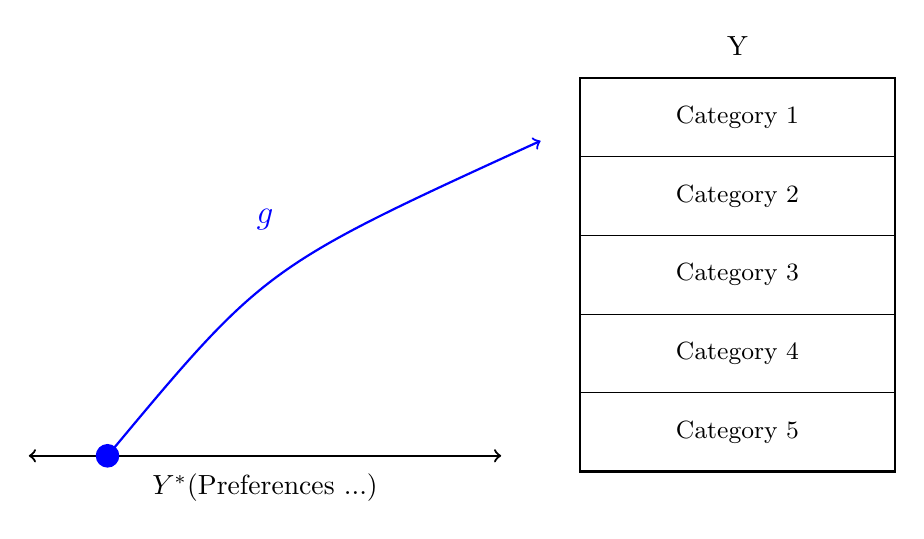
\begin{tikzpicture}
    % Left axis with point and curve
    \draw[thick, <->] (-1,0) -- (5,0);
    \fill[blue] (0,0) circle (0.15cm);
    \draw[blue, thick, ->] (0,0) .. controls (2,2.4) .. (5.5,4);
    \node[blue] at (2,3) {\large $g$};
    \node at (2,-0.4) {$Y^*$(Preferences ...)};

    % Right-hand Y-scale
    \draw[thick] (6,-0.2) rectangle (10.0,4.8);
    \foreach \y in {0.8,1.8,2.8,3.8} { \draw (6,\y) -- (10.0,\y); }

    \node at (8,4.3) {\small Category 1};
    \node at (8,3.3) {\small Category 2};
    \node at (8,2.3) {\small Category 3};
    \node at (8,1.3) {\small Category 4};
    \node at (8,0.3) {\small Category 5};

    \node at (8,5.2) {Y};
    \end{tikzpicture}
\end{frame}

\begin{frame}{Potential Outcome Framework}
    \begin{itemize}
        \item Denote the binary treatment status of individual $d_{i} \in \{0, 1\}$
        \item Denote the potential outcomes in latent preference scale as $Y_{i}^{\ast}(d_{i})$
            \begin{itemize}
                \item $Y_{i}^{\ast}(1) = \tau + \beta X_{i} + \epsilon_{i}$
                \item $Y_{i}^{\ast}(0) = \beta X_{i} + \epsilon_{i}$
            \end{itemize}
        \item Denote the potential outcomes in observed ordinal scale (POO) as $Y_{i}(d_{i}) = g(Y_{i}^{\ast}(d_{i})) \in \{1, \ldots, j,\ldots J\}$
        \item We are interested in the average treatment effect in the latent space (LTE)
            $$
            \begin{aligned}
                LTE &= \mathbb{E}\left[Y^{\ast}(1)\right] - \mathbb{E}\left[Y^{\ast}(0)\right] \\
                &= \tau
            \end{aligned}
            $$ 
    \end{itemize}
\end{frame}

\begin{frame}{LTE with $Y(d_{i})$}
\begin{itemize}
    \item If we knew $Y^{\ast}$, there is not problem
    \item If we knew $g$ and it maps one value of $Y^{\ast}$ to $Y$, then we may get LTE, but this not true in most settings
        $$
            \mathbb{E}\left[g^{-1}(Y_{i}(1))\right] - \mathbb{E}\left[g^{-1}(Y_{i}(0))\right] \neq LTE
        $$ 
    \item Instead, we may identify it up to scale
\end{itemize}
\end{frame}

\begin{frame}{ALTE}
    \begin{itemize}
        \item We can identify the LTE up to scale of a constant if we know or can estimate the distribution of the $\epsilon_{i}$
        \item Suppose the error term has a cdf of $F$
        \item From the model,
            $$
            \begin{aligned}
                \mathbb{P}\left(Y(D) \le j\right) &= \mathbb{P}\left(Y^{\ast} \le \alpha_j \right) \\
            \end{aligned}
            $$  
        \item However, if we scale $Y^{\ast}$ side by a constant, $c$, we still get the same probability
            $$
            \begin{aligned}
                \mathbb{P}\left(Y(D) \le j\right) &= \mathbb{P}\left(Y^{\ast} \le \alpha_j \right) \\
                &= \mathbb{P}\left(c Y^{\ast} \le c \alpha_j\right) \\
            \end{aligned}
            $$  
    \end{itemize}
\end{frame}

\begin{frame}{ALTE}
    \begin{itemize}
        \item Taking account the constant $c$, we can get
            $$
            \begin{aligned}
                F^{-1} ( \mathbb{P}\left( Y (0) & \le j \right) )) - F^{-1} \left( \mathbb{P}\left( Y(1) \le j\right) \right) \\ 
                &= F^{-1}\left( \mathbb{P}\left(c Y^{\ast}(0) \le c\alpha_j\right) \right) - F^{-1} (\mathbb{P}\left(c Y^{\ast}(1) \le c \alpha_{j}\right)) \\
                &= F^{-1}\left( F(c \alpha_j - c \beta X) \right) - F^{-1}_{c \epsilon} (F(c\alpha_{j} - c\beta X - c\tau)\right)) \\
                &= c\tau \\
            \end{aligned}
            $$ 
        \item Good news is similarly we can identify $\beta$ up to the same constant scale too
        \item This enable us to identify LTE anchored on $\beta$ (ALTE)
            $$
                ALTE = \frac{\tau}{\beta}
            $$ 

\end{itemize}
\end{frame}

\begin{frame}{Common Approach}
    \begin{itemize}
        \item Cardinalization of the ordinal outcome
        \item Ordered Logit and Probit
    \end{itemize}
\end{frame}

\begin{frame}{Cardinalization}
    \begin{itemize}
        \item Assume that each responses came from certain numeric value
        \item In other words, the transformation function $g$ will look just like:
            $g = \begin{cases}
                \text{Strongly Diagree} &\quad \text{if } Y^{\ast} = 1\\
                \text{Disagree Somewhat} &\quad \text{if } Y^{\ast} = 2\\
                \text{Neither} &\quad \text{if } Y^{\ast} = 3\\
                \text{Agree Somewhat} &\quad \text{if } Y^{\ast} = 4\\
                \text{Strongly Agree} &\quad \text{if } Y^{\ast} = 5\\
            \end{cases}$
        \item If this is true, we can calculate the average treatment effect by taking the inverse of $g$.
            $$
            \begin{aligned}
                LTE &= \mathbb{E}\left[g^{-1}(Y(1))\right] - \mathbb{E}\left[g^{-1}(Y(0))\right]\\
                &= \mathbb{E}\left[Y^{\ast}(1)\right] - \mathbb{E}\left[Y^\ast(0)\right]
            \end{aligned}
            $$ 
        \item The problem is, the assumption is unlikely and arbitrary
    \end{itemize}
\end{frame}

\begin{frame}{Small Example}
    \begin{table}[ht]
        \centering
        \begin{tabular}{rllll}
            \hline
            & $Y^{\ast}(0)$ & $Y^{\ast}(1)$ & $Y(0)$ & $Y(1)$ \\
            \hline
            A & 1.37 & 0.09 & Agree Somewhat & Disagree Somewhat \\
            B & -0.56 & 1.71 & Disagree Somewhat & Agree Somewhat \\
            C & 0.36 & 0.11 & Neither & Disagree Somewhat \\
            D & 0.63 & 2.22 & Neither & Agree Somewhat \\
            E & 0.4 & 0.14 & Neither & Disagree Somewhat \\
            \hline
        \end{tabular}
    \end{table}
    \begin{itemize}
        \item The LTE in the latent preference space is: $0.41$
    \end{itemize}
\end{frame}

\begin{frame}{Small Example}
    \begin{itemize}
        \item Average Joe may assign 1 to 5 to each responses
    \end{itemize}
    \begin{table}[ht]
        \centering
        \begin{tabular}{rllll}
            \hline
            & $Y^{\ast}(0)$ & $Y^{\ast}(1)$ & $Y_{Joe}(0)$ & $Y_{Joe}(1)$ \\
            \hline
            A & 1.37 & 0.09 & 4 & 2 \\
            B & -0.56 & 1.71 & 2 & 4 \\
            C & 0.36 & 0.11 & 3 & 2 \\
            D & 0.63 & 2.22 & 3 & 4 \\
            E & 0.4 & 0.14 & 3 & 2 \\
            \hline
        \end{tabular}
    \end{table}
    \begin{itemize}
        \item The LTE based on the Joe's cardinalization: $-0.2 \neq 0.41$
    \end{itemize}
\end{frame}

\begin{frame}{Small Example}
    \begin{itemize}
        \item Bold Soyeon comes in and argue that it should be -5, -2, 0, 8, 10 to each responses
    \end{itemize}
    \begin{table}[ht]
        \centering
        \begin{tabular}{rllll}
            \hline
            & $Y^{\ast}(0)$ & $Y^{\ast}(1)$ & $Y_{Soyeon}(0)$ & $Y_{Soyeon}(1)$ \\
            \hline
            1 & 1.37 & 0.09 & 8 & -2 \\
            2 & -0.56 & 1.71 & -2 & 8 \\
            3 & 0.36 & 0.11 & 0 & -2 \\
            4 & 0.63 & 2.22 & 0 & 8 \\
            5 & 0.4 & 0.14 & 0 & -2 \\
            \hline
        \end{tabular}
    \end{table}
    \begin{itemize}
        \item The LTE based on the Soyeon's cardinalization: $0.8 \neq 0.41$
    \end{itemize}
\end{frame}

\begin{frame}{Small Example}
    \begin{itemize}
        \item Smart Jacob finally argue that it should be -5, -2, 0, 8, 10 to each responses
    \end{itemize}
    \begin{table}[ht]
        \centering
        \begin{tabular}{rllll}
            \hline
            & $Y^{\ast}(0)$ & $Y^{\ast}(1)$ & $Y_{Jacob}(0)$ & $Y_{Jacob}(1)$ \\
            \hline
            1 & 1.37 & 0.09 & 6 & -2 \\
            2 & -0.56 & 1.71 & -2 & 6 \\
            3 & 0.36 & 0.11 & 0 & -2 \\
            4 & 0.63 & 2.22 & 0 & 6 \\
            5 & 0.4 & 0.14 & 0 & -2 \\
            \hline
        \end{tabular}
    \end{table}
    \begin{itemize}
        \item The LTE based on the Jacob's cardinalization: $0.4 \approx 0.41$
    \end{itemize}
\end{frame}

\begin{frame}{Ordered Logit and Probit}
    \begin{itemize}
        \item Ordered Logit and Probit assume specific $F$ (Logistic and Standard Normal)
        \item And use maximum likelihood to estimate the coefficients
        \item As we discussed, even we assume the $F$, we only can identify coefficients up to scale
        \item The problem is if $F$ is different from Logistic or Standard Normal, the MLE becomes inconsistent
    \end{itemize}
\end{frame}

\begin{frame}{Alternative: Semiparametric Approach}
    \begin{itemize}
        \item Instead of assuming a specific $F$, we can estimate it from the data using kernel density estimation
        \item For notational ease, let's denote $f(X, \beta) + D^{T}\tau$ as $V$. By the Bayes' rule, $\hat{F}\left(Y \le j \mid V) \right)$ can be expressed as:
        $$
            \hat{F}(Y \le j \mid V) = \frac{\mathbb{P}\left(Y \le j\right) \times g_{1}(V \mid Y \le j)}{\mathbb{P}\left(Y \le j\right) \times g_{1}(V \mid Y \le j) + \mathbb{P}\left(Y > j\right) \times g_{0}(V \mid Y > j)}
        $$, where $g_{0}(\cdot)$ and $g_{0}(\cdot)$ denote conditional density of $V$ given $(Y > j)$ or $(Y \le j)$ respectively. 

        \item Then we can construct a quasi log likelihood function based on $\hat{F}$

    \begin{equation}
        \frac{1}{n} \sum_{i = 1}^{n} \hat{m}(X_{i}) \sum_{j = 0}^{J} 1_{\{ Y = j \}} \log \left[ \hat{\mathbb{P}}\left(Y \le j \mid X_{i}, \beta, D_{i}, \tau \right) - \hat{\mathbb{P}}\left( Y \le j-1 \mid X_{i}, \beta, D_{i}, \tau)\right) \right]
    \end{equation}
    \end{itemize}

\end{frame}

%\begin{frame}{Problem 1: Interpretation}
%    Q: (Respondent’s country) should limit the import of foreign products in order to protect its national economy.”
%        \includegraphics[width=0.95\textwidth]{../figures/interpretation1.pdf}
%\end{frame}
%
%\begin{frame}{Problem 1: Interpretation}
%    Q: (Respondent’s country) should limit the import of foreign products in order to protect its national economy.”
%        \includegraphics[width=0.95\textwidth]{../figures/interpretation2.pdf}
%\end{frame}
%
%\begin{frame}{Problem 1: Interpretation}
%    Q: (Respondent’s country) should limit the import of foreign products in order to protect its national economy.”
%        \includegraphics[width=0.95\textwidth]{../figures/interpretation3.pdf}
%\end{frame}
%
%\begin{frame}{Problem 2: Distribution}
%        \includegraphics[width=0.95\textwidth]{../figures/distribution0.pdf}
%\end{frame}
%
%\begin{frame}{Problem 2: Distribution}
%        \includegraphics[width=0.95\textwidth]{../figures/distribution1.pdf}
%\end{frame}
%
%\begin{frame}{Problem 2: Distribution}
%        \includegraphics[width=0.95\textwidth]{../figures/distribution2.pdf}
%\end{frame}
%
%\begin{frame}{Problem 2: Distribution}
%        \includegraphics[width=0.95\textwidth]{../figures/distribution3.pdf}
%\end{frame}
%
%\begin{frame}{Problem 2: Distribution}
%        \includegraphics[width=0.95\textwidth]{../figures/distribution4.pdf}
%\end{frame}
%
%\begin{frame}{Problem 2: Distribution}
%        \includegraphics[width=0.95\textwidth]{../figures/distribution5.pdf}
%\end{frame}
%
%\begin{frame}{Problem 3: Imprecise Measure}
%    \begin{itemize}[<+->]
%        \item Usually, education (years of schooling), income, assets are included in the regression either as independent variables or as control variables
%        \item For privacy issues these are usually measured in brackets
%        \item Researchers do not know the exact value, but only observe the lower and the upper bounds
%            \\ INCOME
%            \\ \textit{\$5,000 -- \$10,000}
%    \end{itemize}
%\end{frame}


% \begin{frame}{Previous Works}
%         \begin{tabular}{|c|c|c|c|}
%             \hline
%             & Interpretation & Distribution & Imprecise \\ \hline
%             \begin{tabular}[c]{@{}c@{}} Anchored Vignettes \\ {\tiny \citep{King2004a, King2007a}}
%             \end{tabular}  & $\checkmark$ &   &  \\ \hline
%             \begin{tabular}[c]{@{}c@{}}Semiparametric\\ {\tiny \citep{Lewbel2000a, Lee1992a, Liu2024a}}  \\ Sensitivity Analysis \\ {\tiny \citep{Bloem2022a}}\end{tabular} & $\checkmark$     & $\checkmark$   &                     \\ \hline
%         \end{tabular}
% \end{frame}
%
% \begin{frame}{This Paper}
%     \begin{table}[]
%         \begin{tabular}{|c|c|c|c|}
%             \hline
%             & Interpretation & Distribution & Imprecise \\ \hline
%             Anchored Vignettes                                                             & $\checkmark$     &              &                     \\ \hline
%             \begin{tabular}[c]{@{}c@{}}Semiparametric\\ Sensitivity Analysis\end{tabular} & $\checkmark$     & $\checkmark$   &                     \\ \hline
%                 \begin{tabular}[c]{@{}c@{}}Semiparametric\\ Partial Identification \\ {\tiny\cite{Manski2002a, Wang2022a}} \end{tabular} & $\checkmark$     & $\checkmark$   & $\checkmark$          \\ \hline
%         \end{tabular}
%     \end{table}
% \end{frame}
%
% \begin{frame}{Problem Setting}
%     True DGP:
%     \begin{equation}
%         Y^{\ast} = X^{T}\beta_{1} + v^{T}\beta_{2} + \epsilon
%     \end{equation}
%     Observation:
% \begin{equation}
%     Y = \begin{cases}
%         0 & Y^{\ast} \le 0 \\
%         1 & 0 \le Y^{\ast} \le \alpha_{1} \\
%         \vdots &  \\
%         k & \alpha_{k-1} \le Y^{\ast} \le \alpha_{k} \\
%     \end{cases}
% \end{equation}
% Also, we do not observe $v$ directly, the lower bound of $v_{0}$ and the upper bound of $v_{1}$ 
% \end{frame}
%
% \begin{frame}{Assumptions}
%     \begin{assumption}[1]
%         $Q_{\tau}(\epsilon \mid X, v) = 0$
%     \end{assumption}
%
%     \begin{assumption}[2]
%         $\mathbb{P}\left(\epsilon \mid X, v, v_{0}, v_{1}\right) = \mathbb{P}\left(\epsilon \mid X, v\right)$
%     \end{assumption}
%
%     \begin{assumption}[3]
%         $\beta_{2} > 0$
%     \end{assumption}
% \end{frame}
%
% \begin{frame}{GMMS Estimator}
%     Let $\lambda_{mn}(\cdot) = \mathbb{1}_{\{ \mathbb{P}\left( Y_i > m \mid X_i, V_{1 i}, V_{0 i}\right) > (1 - \tau)\}}$
% \begin{equation*}
%     \begin{aligned}
%         \Theta_n &= \{ b: S_{n}(b) \ge \max_{C \in \mathcal{B}} S_{n}(c) - \varepsilon_{n}\}\\
%     \end{aligned}
% \end{equation*}
% , where
%
% \begin{multline*}
% %\begin{equation}
%     S_n(b^s) = \frac{1}{n} \sum_{i=1}^n \sum_{m=1}^{M-1} \biggl(\mathbb{P}(Y_i > m \mid X_i, V_{0i}, V_{1i}) - (1 - \tau)\biggl) \\
%     \biggl[ \lambda_{mn}(X_i, V_{0i}, V_{1i}) \cdot \text{sgn}(\tilde{X}'_i b + V^1_i + b_{1m}) + \\
%     (1 - \lambda_{mn}(X_i, V_{0i}, V_{1i})) \cdot \text{sgn}(\tilde{X}'_i b + V_{0i} + b_{1m}){\biggl]}
% %\end{equation}
% \end{multline*}
%     , for some $\varepsilon_{n} = \frac{\ln(n)}{n} > 0$.
%
% \end{frame}

\begin{frame}{Simulation}
\begin{figure}
    \begin{tabular}{cc}
        \includegraphics[width=0.45\textwidth]{../figures/bias_tdis.pdf} & \includegraphics[width=0.45\textwidth]{../figures/rmse_tdis.pdf}\\
        (a) & (b)
    \end{tabular}
    \caption{Monte Carlo Simulation Results: t-distribution Error}
\end{figure}
\end{frame}

\end{document}
